\chapter{Πίνακες μετασχηματισμών στο χώρο τριών διαστάσεων}

\section{Γεωμετρικοί μετασχηματισμοί}

\subsection{Μεταφορά}

\begin{figure}[hbt]
  \begin{center}
	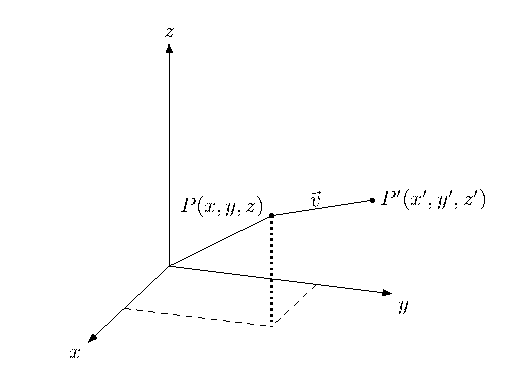
\includegraphics[scale=1]{Chapter3/point-transformation.pdf}
  \end{center}
  \caption{Μεταφορά σημείου σε τρισδιάστατες συντεταγμένες}
\end{figure}



Έστω \( V = (t_x, t_y, t_z) \) τότε \( P' = T_v(P) \) με \( x' = x + t_x \), \( y' = y + t_y \), \( z' = z + t_z \). Το σημείο \((x, y, z)\) σε ομογενείς συντεταγμένες γράφεται:

\[
\begin{bmatrix}
x \\
y \\
z \\
1
\end{bmatrix}
\]

Ο πίνακας μετασχηματισμού της μεταφοράς θα είναι:

\[
T_v =
\begin{bmatrix}
1 & 0 & 0 & t_x \\
0 & 1 & 0 & t_y \\
0 & 0 & 1 & t_z \\
0 & 0 & 0 & 1
\end{bmatrix}
\]

\subsubsection*{5.1.2 Μετασχηματισμός κλίμακας}

\( P' = S_{S_x, S_y, S_z}(P) \) με \( x' = s_x x \), \( y' = s_y y \) και \( z' = s_z z \)

Ο πίνακας μετασχηματισμού είναι:

\[
S_{S_x, S_y, S_z} = 
\begin{bmatrix}
s_x & 0 & 0 & 0 \\
0 & s_y & 0 & 0 \\
0 & 0 & s_z & 0 \\
0 & 0 & 0 & 1
\end{bmatrix}
\]


%%%%%%%%%%2


\[
S_{S_x,S_y,S_z} = 
\begin{bmatrix}
S_x & 0 & 0 & 0 \\
0 & S_y & 0 & 0 \\
0 & 0 & S_z & 0 \\
0 & 0 & 0 & 1
\end{bmatrix}
\]

\section{Στροφή}

Στον χώρο τριών διαστάσεων για τη στροφή ενός αντικειμένου απαιτούνται δύο παράμετροι:

\begin{itemize}
    \item α) η γωνία στροφής $\theta$ και
    \item β) ο άξονας περιστροφής του αντικειμένου.
\end{itemize}

Οι "κανονικές" στροφές ορίζονται στον χώρο σαν στροφές γύρω από τους θετικούς άξονες $x$, $y$ και $z$.

Για την περίπτωση του θετικού άξονα $z$ έχουμε εάν το σημείο είναι στο επίπεδο $xOy$:

\begin{center}
\begin{tabular}{c}
$xOy$ \\
\hline
$z$ \\
$0$ \\
$P' (x', y', 0)$ \\
$P (x, y, 0)$ \\
\end{tabular}
\end{center}

\begin{figure}[h]
\centering
\caption{Σχήμα 5.2}
\end{figure}

Με βάση το κεφάλαιο 3 έχουμε:

\begin{itemize}
    \item α) Στροφή γύρω από τον άξονα $z$.

    \[
    P' = R_{\theta,z}(P)
    \]
    με
    \[
    x' = x \cos \theta - y \sin \theta, \quad y' = x \sin \theta + y \cos \theta, \quad z' = z
    \]
    ο αντίστοιχος μετασχηματισμός είναι:
    \[
    R_{\theta,z} = 
    \begin{bmatrix}
    \cos \theta & -\sin \theta & 0 & 0 \\
    \sin \theta & \cos \theta & 0 & 0 \\
    0 & 0 & 1 & 0 \\
    0 & 0 & 0 & 1
    \end{bmatrix}
    \]

    \item β) Στροφή γύρω από τον άξονα $y$.

    \[
    P' = R_{\theta,y}(P)
    \]
    με
    \[
    x' = x \cos \theta + z \sin \theta, \quad y' = y, \quad z' = -x \sin \theta + z \cos \theta
    \]
    και αντίστοιχο μετασχηματισμό:
    \[
    R_{\theta,y} = 
    \begin{bmatrix}
    \cos \theta & 0 & \sin \theta & 0 \\
    0 & 1 & 0 & 0 \\
    -\sin \theta & 0 & \cos \theta & 0 \\
    0 & 0 & 0 & 1
    \end{bmatrix}
    \]
\end{itemize}


%%%%%%%%%%3 

\[
R_{\theta, y} = 
\begin{bmatrix}
\cos \theta & 0 & \sin \theta & 0 \\
0 & 1 & 0 & 0 \\
-\sin \theta & 0 & \cos \theta & 0 \\
0 & 0 & 0 & 1
\end{bmatrix}
\]

\subsection{ Στροφή γύρω από τον άξονα \( x \)}

\[
P' = R_{\theta, x}(P)
\]
με
\[
x' = x, \quad y' = y \cos \theta - z \sin \theta, \quad z' = y \sin \theta + z \cos \theta
\]
και:
\[
R_{\theta, x} = 
\begin{bmatrix}
1 & 0 & 0 & 0 \\
0 & \cos \theta & -\sin \theta & 0 \\
0 & \sin \theta & \cos \theta & 0 \\
0 & 0 & 0 & 1
\end{bmatrix}
\]

\section{Συμμετρία ως προς επίπεδο}

Δίνουμε τους αντίστοιχους πίνακες μετασχηματισμών:

\[
M_{x, y} = 
\begin{bmatrix}
1 & 0 & 0 & 0 \\
0 & 1 & 0 & 0 \\
0 & 0 & -1 & 0 \\
0 & 0 & 0 & 1
\end{bmatrix}
\]

\[
M_{x, z} = 
\begin{bmatrix}
1 & 0 & 0 & 0 \\
0 & -1 & 0 & 0 \\
0 & 0 & 1 & 0 \\
0 & 0 & 0 & 1
\end{bmatrix}
\]

\[
M_{y, z} = 
\begin{bmatrix}
-1 & 0 & 0 & 0 \\
0 & 1 & 0 & 0 \\
0 & 0 & 1 & 0 \\
0 & 0 & 0 & 1
\end{bmatrix}
\]


%%%%%%%%%%4

\subsection*{Αντίστροφοι μετασχηματισμοί}

Για τους αντίστροφους μετασχηματισμούς ισχύει:

\[
T^{-1}_{V} = T_{-V}, \quad R^{-1}_{\theta} = R_{-\theta}, \quad S^{-1}_{S_X,S_Y,S_Z} = S_{\frac{1}{S_X}, \frac{1}{S_Y}, \frac{1}{S_Z}}
\]

\subsection{Μετασχηματισμοί αξόνων συντεταγμένων}

\begin{figure}[h]
\centering
\caption{Σχήμα 5.3}
\end{figure}

Στην περίπτωση της παράλληλης μεταφοράς των αξόνων συντεταγμένων κατά διάνυσμα \( v = (t_x, t_y, t_z) \) έχουμε για τις νέες συντεταγμένες \( (x', y', z') \) του σημείου \( P(x, y, z) \):

\[
x' = x - t_x, \quad y' = y - t_y, \quad z' = z - t_z
\]

Άρα ο μετασχηματισμός \( T_V \) θα είναι ο αντίστοιχος του \( T_{-V} \) γεωμετρικού μετασχηματισμού.

Αντί των πινάκων συντεταγμένων θα δώσουμε εδώ συνοπτικά τις αντιστοιχίες μεταξύ μετασχηματισμών αξόνων συντεταγμένων και γεωμετρικών.

\begin{itemize}
    \item Μεταφορά:  
    \( T_V \leftarrow T_{-V} \)

    \item Μετασχηματισμός κλίμακας:  
    \( S_{S_X,S_Y,S_Z} \leftarrow S_{\frac{1}{S_X}, \frac{1}{S_Y}, \frac{1}{S_Z}} \)

    \item Στροφή:  
    \( R_{\theta} \leftarrow R_{-\theta} \quad R_{\theta,X} \leftarrow R_{-\theta,X} \)

    \( R_{\theta,Y} \leftarrow R_{-\theta,Y} \)

    \( R_{\theta,Z} \leftarrow R_{-\theta,Z} \)
\end{itemize}

Για τους αντίστροφους τέλος μετασχηματισμούς αξόνων συντεταγμένων ισχύει:

\[
T^{-1}_{V} = T_{-V}, \quad R^{-1}_{\theta} = R_{-\theta}, \quad S^{-1}_{S_X,S_Y,S_Z} = S_{\frac{1}{S_X}, \frac{1}{S_Y}, \frac{1}{S_Z}}
\]

 
%%%%%%%% 5
Επίσης εδώ πρέπει να αναφερθεί ότι όπως και στην περίπτωση των δύο συντεταγμένων έτσι και εδώ, πεπλεγμένοι μετασχηματισμοί αντιμετωπίζονται με τη διαδικασία της σύνθεσης συναρτήσεων η οποία εδώ ταυτίζεται με τον πολλαπλασιασμό πινάκων. Αναφέρουμε το παρακάτω παράδειγμα:

Να υπολογιστεί ο πίνακας μετασχηματισμού \( T \) για την περίπτωση στροφής γύρω από τον άξονα \( x \) κατά γωνία \( \theta_x \) και στη συνέχεια στροφή ως προς \( y \) κατά γωνία \( \theta_y \).

\[
T = R_{\theta_y, y} \cdot R_{\theta_x, x}
\]

\[
\begin{bmatrix}
C_{(r+1)^2} \\
0 \\
\end{bmatrix}
=
\begin{bmatrix}
\cos \theta_y & 0 & \sin \theta_y & 0 \\
0 & 1 & 0 & 0 \\
-\sin \theta_y & 0 & \cos \theta_y & 0 \\
0 & 0 & 0 & 1
\end{bmatrix}
\begin{bmatrix}
1 & 0 & 0 & 0 \\
0 & \cos \theta_x & -\sin \theta_x & 0 \\
0 & \sin \theta_x & \cos \theta_x & 0 \\
0 & 0 & 0 & 1
\end{bmatrix}
=
\begin{bmatrix}
\cos \theta_y & \sin \theta_y \sin \theta_x & \sin \theta_y \cos \theta_x & 0 \\
0 & \cos \theta_x & -\sin \theta_x & 0 \\
-\sin \theta_y & \cos \theta_y \sin \theta_x & \cos \theta_y \cos \theta_x & 0 \\
0 & 0 & 0 & 1
\end{bmatrix}
\]

\section{ Παραδείγματα μετασχηματισμών στο χώρο}

\begin{example}
	Ορίζουμε ως "καμπή" την περιστροφή γύρω από τον άξονα \( x \) και στη συνέχεια γύρω από τον άξονα \( y \). 
	
	\begin{itemize}
	    \item Βρείτε τον πίνακα καμπής \( T_k \).
	    \item Εξετάστε εάν παίζει ρόλο η σειρά με την οποία εκτελείται η περιστροφή.
	\end{itemize}
\end{example}

\begin{solution}
	

Τα ακόλουθα βήματα καθορίζουν τον ζητούμενο πίνακα.

\begin{itemize}
    \item \textbf{Βήμα 1:} Στροφή κατά γωνία \( \theta_x \) ως προς τον άξονα \( x \).

    Βασικός πίνακας μετασχηματισμού: \( R_{\theta_x, x} \).

    \item \textbf{Βήμα 2:} Στροφή κατά γωνία \( \theta_y \) ως προς τον άξονα \( y \).

    Βασικός πίνακας μετασχηματισμού: \( R_{\theta_y, y} \).

    Ο ζητούμενος πίνακας θα προκύψει σαν σύνθεση των παραπάνω βασικών μετασχηματισμών.
\end{itemize}

\end{solution}


%%%%%%%%%% 6

\[
T_k = R_{\theta_y, y} \cdot R_{\theta_x, x} =
\]

\[
\begin{bmatrix}
\cos \theta_y & 0 & \sin \theta_y & 0 \\
0 & 1 & 0 & 0 \\
-\sin \theta_y & 0 & \cos \theta_y & 0 \\
0 & 0 & 0 & 1
\end{bmatrix}
\begin{bmatrix}
1 & 0 & 0 & 0 \\
0 & \cos \theta_x & -\sin \theta_x & 0 \\
0 & \sin \theta_x & \cos \theta_x & 0 \\
0 & 0 & 0 & 1
\end{bmatrix}
\]

\[
= 
\begin{bmatrix}
\cos \theta_y & \sin \theta_y \sin \theta_x & \sin \theta_y \cos \theta_x & 0 \\
0 & \cos \theta_x & -\sin \theta_x & 0 \\
-\sin \theta_y & \cos \theta_y \sin \theta_x & \cos \theta_y \cos \theta_x & 0 \\
0 & 0 & 0 & 1
\end{bmatrix}
\]

(β) Εάν εκτελεστούν οι παραπάνω μετασχηματισμοί με αντίθετη σειρά θα προκύψει ο ακόλουθος πίνακας:

\[
T_k = R_{\theta_x, x} \cdot R_{\theta_y, y} =
\]

\[
\begin{bmatrix}
\cos \theta_y & 0 & \sin \theta_y & 0 \\
\sin \theta_x \sin \theta_y & \cos \theta_x & -\sin \theta_x \cos \theta_y & 0 \\
-\cos \theta_x \sin \theta_y & \sin \theta_x & \cos \theta_x \cos \theta_y & 0 \\
0 & 0 & 0 & 1
\end{bmatrix}
\]

Παρατηρούμε ότι ο νέος πίνακας διαφέρει από αυτόν του ερωτήματος (α) επομένως παίζει σημαντικό ρόλο η σειρά με την οποία εκτελείται η περιστροφή.

\begin{example}
Προσδιορίστε το μετασχηματισμό \( A_n \) που ευθυγραμμίζει δοσμένο διάνυσμα \( V \) με το μοναδιαίο διάνυσμα \( k \) κατά μήκος του θετικού μέρους του άξονα των \( z \).

\end{example}
